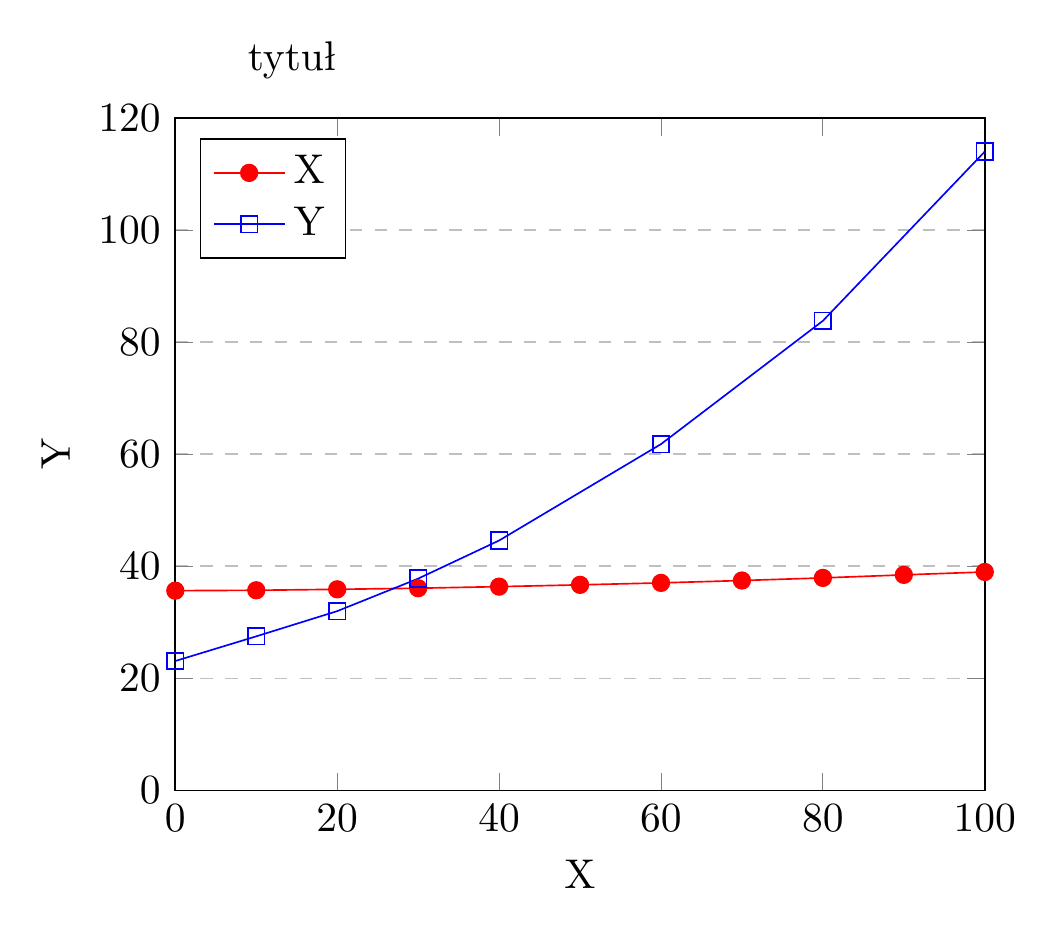
\begin{tikzpicture}[scale=1.5]
    \begin{axis}[
    title={tytuł},
    title style={text width=16em},
    xlabel={X },
    ylabel={Y},
    xmin=0,xmax=100,
    ymin=0,ymax=120,
    legend pos=north west,
    ymajorgrids=true,grid style=dashed
    ]
    
    \addplot[color=red,mark=*]
    coordinates {
    (0,35.65)
    (10,35.72)
    (20,35.89)
    (30,36.09)
    (40,36.37)
    (50,36.69)
    (60,37.04)
    (70,37.46)
    (80,37.93)
    (90,38.47)
    (100,38.99)
    };
    
    \addplot[color=blue,mark=square]
    coordinates {
    (0,23.1)
    (10,27.5)
    (20,32)
    (30,37.8)
    (40,44.6)
    (60,61.8)
    (80,83.8)
    (100,114)
    };
    
    \legend{X,Y}
    \end{axis}
    \end{tikzpicture}
    
    
